

\noindent
Utilizing high‐resolution floodplain maps of Europe provided by \citet{dottori_et_al_2022}, I propose and develop a time-invariant flood risk index that is used to stratify the econometric analysis and guide sample selections. I choose the floodplain map with RP100 floods, indicating the extent of flooding that is statistically expected to be equaled or exceeded on average once every 100 years, a standard return period used in insurance and urban planning. I overlay the RP100 raster (GeoTIFF) data—a grid of 90m × 90m cells, each with a continuous value of water depth (in meters)—onto the polygons of all communes in metropolitan France. Counting how many of the raster cells fall within the boundaries of a commune, and then converting cell counts to surface areas, allows me to compute the percentage share of a commune's total area that is exposed to varying intensities of flood risk. Following categorization schemes used by the European Commission’s \href{https://drmkc.jrc.ec.europa.eu/risk-data-hub#/}{Risk
 Data Hub} and in the PESETA reports, I classify exposure intensity of each raster cell into four bands: $(0–0.5m]$, $(0.5–1.5m]$, $(1.5–3m]$, and $>3m$. The distribution of water depth values is heavily right-skewed, as shown in Figure \ref{fig:raster_values_distrib}. For each commune, the risk index is simply built as the sum of four variables, capturing the proportion of the commune’s total surface falling into each of the four depth bands, and excluding “unflooded” remainder. The risk index thus ranges from 0 to 100, and is plotted in Figure \ref{fig:risk_index}; it can be conceived as the share of each commune’s surface that is colored in purple in Figure \ref{fig:raster_unbinned}. Several flood risk or exposure indices are used in the academic literature—alongside \cite{indaco2024adapting} and \cite{hussain2024flooding}. Other indices range from global event-based \citep{okazawa2011development}, local exposure-vulnerability \cite{anindita2020flood}, GIS susceptibility models, to composite social-exposure indices and macro-scale global indices (WorldRiskIndex). These indices go in the direction of the damage function in \cite{carleton2022valuing} and, more specifically for our application, the damage functions in \cite{bilal2023anticipating}.

This measure of flood hazard could be refined in several ways. Rather than relying on a simple sum of flooded area across intensity categories, a weighted sum—placing greater emphasis on more severe flooding—would better reflect the nonlinear relationship between water depth and economic damage often observed in engineering and insurance data \cite{ballocci2024econometric}. For example, a commune that is 30\% flooded at 2 meters likely faces far greater losses than one that is 100\% flooded at 5 cm. Similarly, exploiting multiple return periods (e.g., RP10 vs. RP500) would allow the index to capture temporal variation in exposure, distinguishing between persistently exposed areas and those facing latent, tail risks. These “risk-jumpers” can be identified by subtracting RP10 from RP500 flood depths—a difference that preliminary analysis has shown to be minimal in most regions but notable in places like the Loire Valley around the city of Orléans, highlighting the importance of such hazard maps in informing investments in resilience across France. As explained in Section \ref{ch: discussion}, to improve precision of my estimates, beyond the risk index I include other time-invariant covariates in my specification, such as the share of establishments covered by EAIP (Figure \ref{fig:eaip_map}) and commune median revenue. I also test other covariates that could have been included directly in the index. Table \ref{tab:pscore_logit} shows results.

%Table X reports the share of communes classified as “risk-jumpers” (large RP500 vs. RP10 exposure) by region versus those under chronic risk, as well as other statistics around the risk index (including correlation with CatNat events). 

Finally, in integrated structural models of climate change, a flood risk index at the commune level could act as an amenity shifter that affects the relative desirability of locations. Households and firms are assumed to sort spatially based on wages, prices, and local amenities, influencing spatial sorting and long-run equilibrium under evolving climate risk. By simulating these equilibria under different flood scenarios (e.g., comparing RP10 vs. RP500), the model can generate forward-looking predictions of where people and firms are likely to concentrate or retreat. %offering a powerful tool for long-term planning and adaptation policy.
\vspace{0.3cm}

\begin{figure}[!htbp]

  \centering
  % first subfigure at 49% of text width
  \caption{\textbf{Figure \ref{fig:raster_flood}:} Hazard exposure - Flood raster data (RP100)}
  \label{fig:raster_flood}
  \begin{subfigure}[b]{0.44\textwidth}
    \centering
    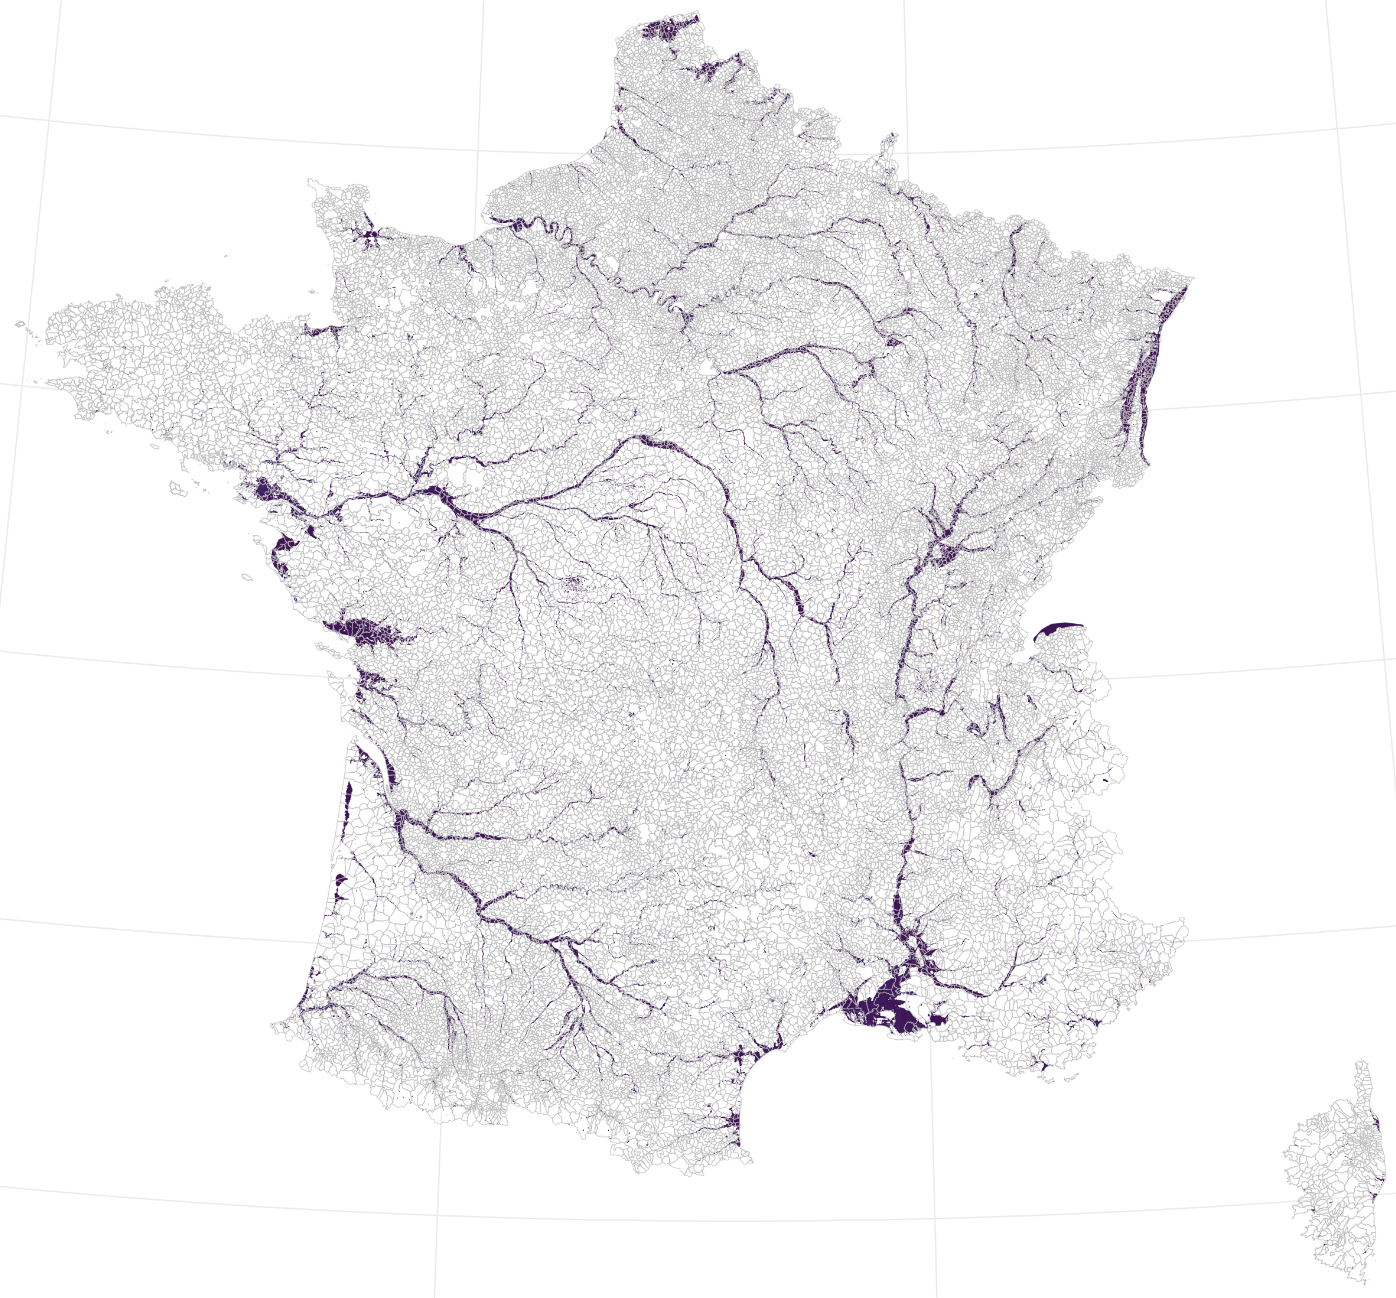
\includegraphics[width=\linewidth]{figures/Data/Raster Unbinned.png}
    \subcaption{Extensive margin of ex-ante risk}
    \label{fig:raster_unbinned}
  \end{subfigure}%i
  % tiny horizontal skip, then second
  \hspace{0.02\textwidth}%
  \begin{subfigure}[b]{0.536\textwidth}
    \centering
    
\includegraphics[width=\linewidth]{figures/Data/Raster Binned.png}
    \subcaption{Intensive margin of ex-ante risk}
    \label{fig:raster_binned}
\end{subfigure}



\end{figure}


\begin{figure}[!htbp]
    \centering
    \caption{\textbf{Figure \ref{fig:raster_values_distrib}:} Histogram of RP100 flood‐depth values at 90m×90m resolution}
    \label{fig:raster_values_distrib}
    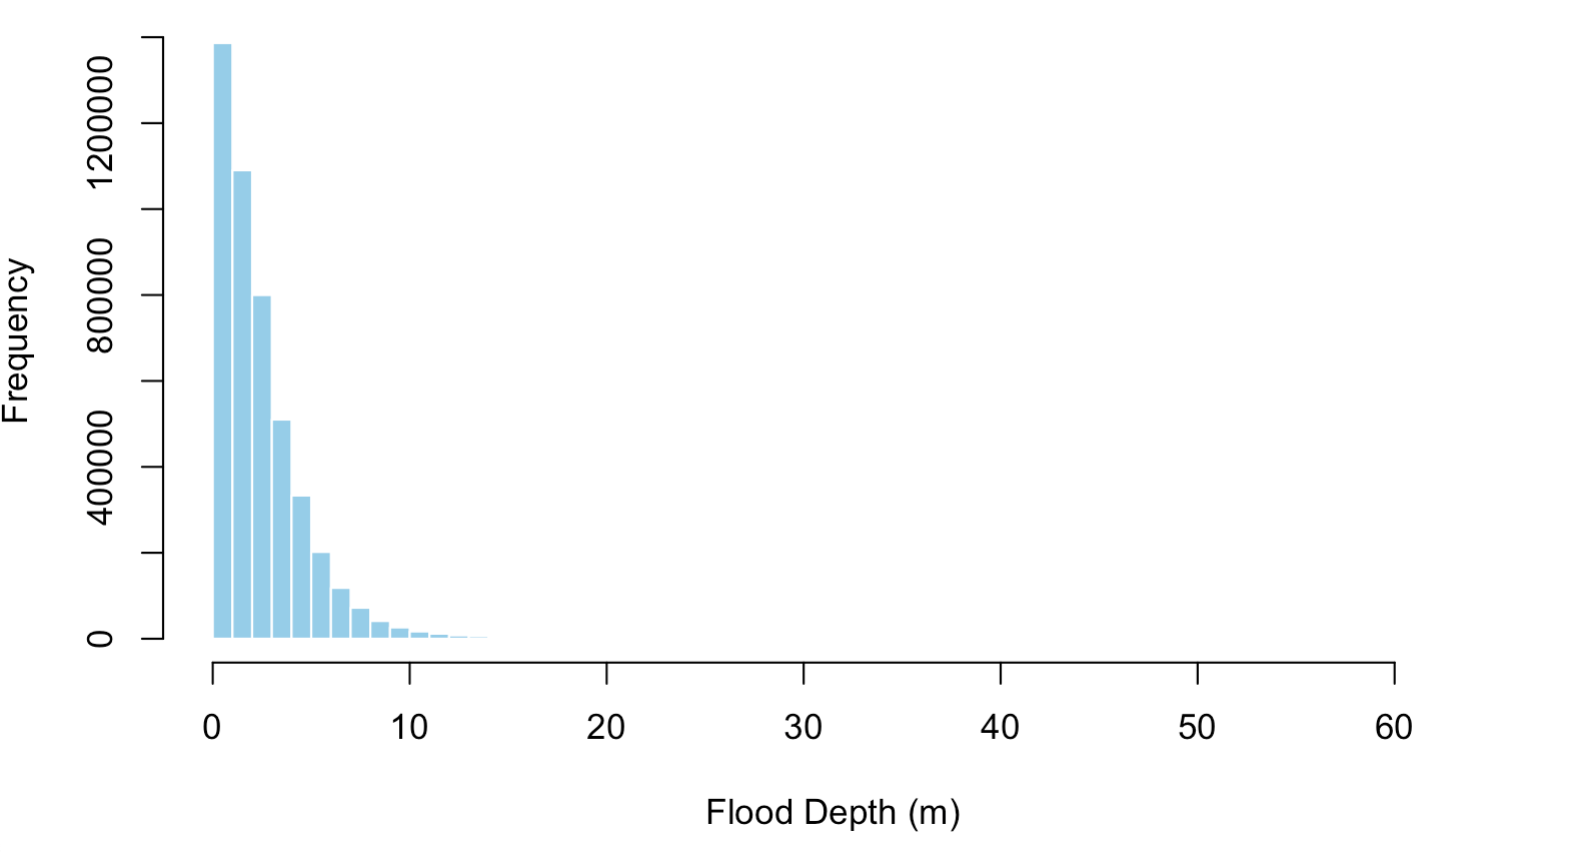
\includegraphics[width=0.7\textwidth]{figures/Data/Raster depth values.png}
    \caption*{\raggedright\textit{Note}: The distribution is markedly right-skewed: the vast majority of pixels record minimal inundation, while a small tail captures the comparatively rare, deeper flood depths. Furthermore, 90\% of all flooded cells fall between 0.07 and 3 meters in water depth.}
    
    \end{figure}


\begin{figure}[!htbp]
    \centering
    \caption{\textbf{Figure \ref{fig:risk_disribu}:} Histogram of Flood Risk Index values at commune level}
    \label{fig:risk_disribu}
    
    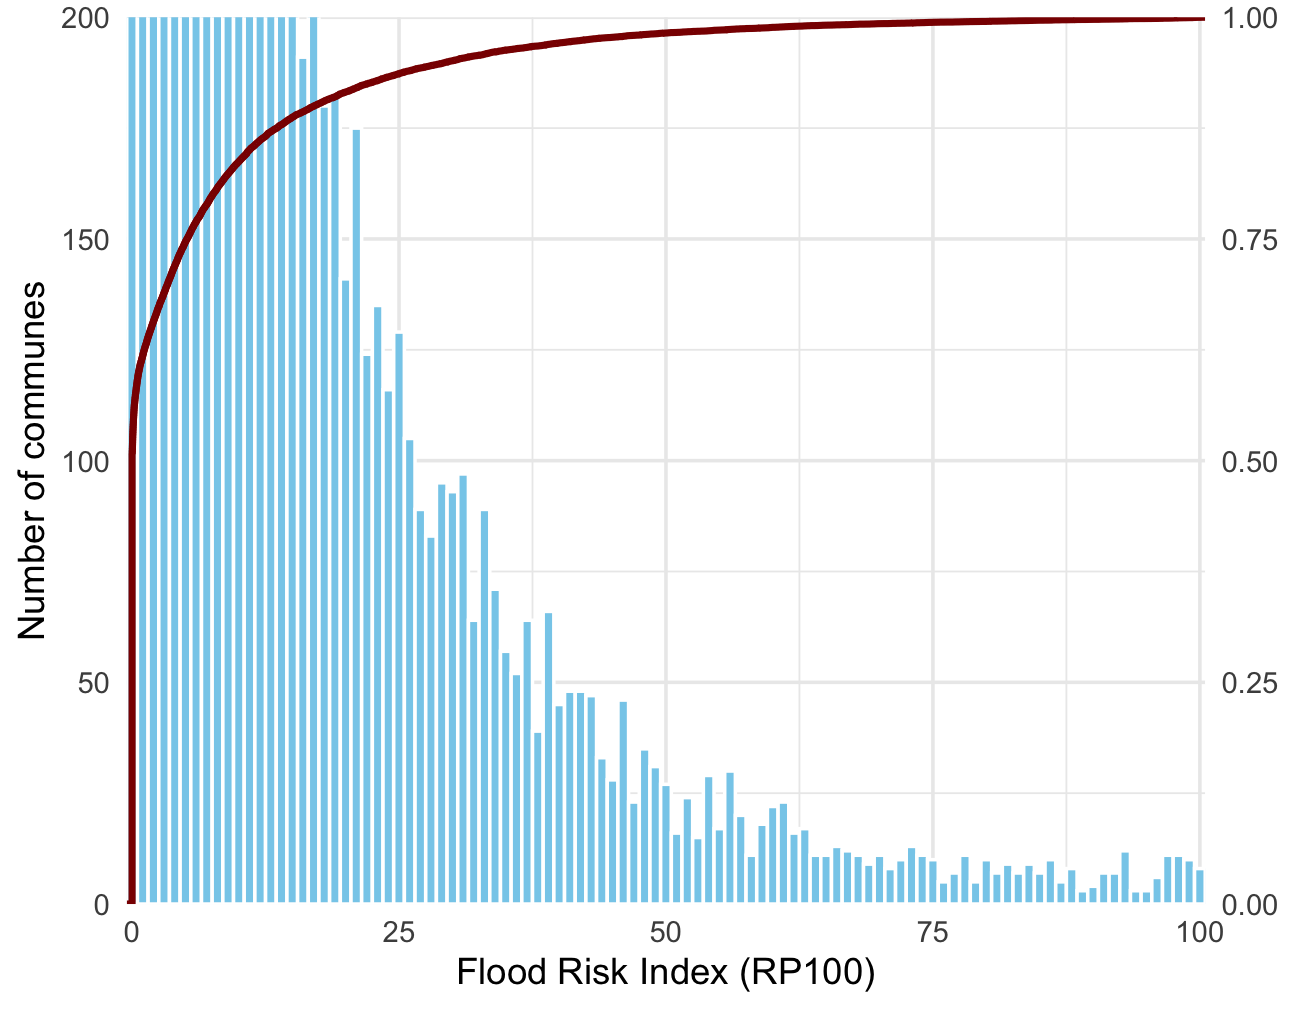
\includegraphics[width=0.7\textwidth]{figures/Data/disribution risk index.png}
    %\caption*{\raggedright\textit{Note: The distribution of the index}}
    
    \end{figure}











